\documentclass[a4paper,12pt]{book}

\usepackage{ZeroSeven}
\usepackage{ltablex}
\titlepage{}

\author{Ludovico Brocca}
\date{2018-12-19}
\intestazioni{
\includegraphics[scale=0.3]{images/logo_intestazione}}
\pagestyle{myfront}
\begin{document}
\begin{titlepage}
	\centering
	{\huge\bfseries MegAlexa \par}
	Arricchitore di skill di Amazon Alexa
	\line(1,0){350} \\
	{\scshape\LARGE Analisi Dei Requisiti \par}
	\vspace{1cm}
	{\scshape Gruppo ZeroSeven \par}
	\logo
	%devono essere compilati questi campi ogni volta
	\begin{tabular}{c|c}
		{\hfill \textbf{Versione}} 			& 0.0.6				\\
		{\hfill\textbf{Data Redazione}} 	& 2018-12-19		\\ 
		{\hfill\textbf{Redazione}} 			&  		Ludovico Brocca \\ & Matteo Depascale	\\	
		{\hfill\textbf{Verifica}} 				&  	Nome Cognome			\\ 
		{\hfill\textbf{Approvazione}} 		&  		Nome Cognome			\\ 
		{\hfill\textbf{Uso}} 					& 		Esterno		\\ 
		{\hfill\textbf{Distribuzione}} 			& 			Prof. Tullio Vardanega \\ & Prof. Riccardo Cardin \\ & Gruppo ZeroSeven		\\ 
		{\hfill\textbf{Email di contatto}} & zerosevenswe@gmail.com \\
	\end{tabular}
\end{titlepage}
	

	
	\label{LastFrontPage}
	\newpage	
	\begin{center}
	\textbf{Registro delle modifiche}
	\end{center}
	\begin{center}
		\begin{tabularx}{\textwidth}{|c|c|X|X|c|}
			\hline
			\textbf{Versione} & \textbf{Data} & \textbf{Descrizione} & \textbf{Autore} & \textbf{Ruolo} \\ 
			\hline
			3.0.0 & 2019-04-11 & Approvazione per il rilascio RQ & Ludovico Brocca & Responsabile \\
			\hline
			2.1.0 & 2019-04-09 & Verifica documento & Ludovico Brocca & Verificatore \\
			\hline
			2.0.6 & 2019-04-08 & Aggiunto riferimento metriche alla sezione \S\ref{MetricheObbiettivi} &Matteo depascale & Amministratore \\
			\hline 
			2.0.5 & 2019-04-08 & Modifica sezioni \S\ref{Verifica}  e \S\ref{Validazione} & Matteo depascale & Amministratore \\
			\hline
			2.0.4 & 2019-04-08 & Aggiunti comandi personalizzati alla sezione \S\ref{NormeRedazionali} &Matteo depascale & Amministratore \\
			\hline
			2.0.3 & 2019-04-04 & Aggiunta voci a \S\ref{ListaControllo} & Matteo depascale & Amministratore \\
			\hline
			2.0.2 & 2019-04-01 & Stesura sezioni \S\ref{DiagrammiDelleClassi}, \S\ref{DiagrammiPackage}, \S\ref{DiagrammiSequenza} e \S\ref{DiagrammiAttivita}  & Bianca Andreea Ciuche & Amministratore \\
			\hline
			2.0.1 & 2019-03-23 & Modifica \ref{Documentazione fornita} Corretti numeri di sezione & Bianca Andreea Ciuche & Amministratore \\
			\hline
			2.0.0 &2019-03-07 & Approvazione per il rilascio & Gian Marco Bratzu& Responsabile\\
			\hline
			1.2.0 &2019-03-02 & Verifica documento &Andrea Deidda& Verificatore\\
			\hline
			1.1.2 &2019-02-13 &Stesura \S\ref{calcoloOre} &Ludovico Brocca& Amministratore\\
			\hline
			1.1.1 &2019-02-13 &Modifica\S \ref{anDinamica} &Ludovico Brocca& Amministratore\\
			\hline
			1.1.0 &2019-02-07 &Verifica \S\ref{processo}, \ref{metriche}, \S\ref{progettazione} &Gian Marco Bratzu& Verificatore\\
			\hline
			1.0.4 &2019-02-04&Stesura \S\ref{processo}&Ludovico Brocca& Analista\\
			\hline
			1.0.3 & 2019-02-03 & Modifica \S\ref{metriche} & Stefano Zanatta & Amministratore\\
			\hline
			1.0.2 & 2019-02-02 & Stesura \S\ref{metriche} & Bianca Andreea Ciuche & Amministratore\\
			\hline
			1.0.1 & 2018-01-12 & Stesura \S\ref{progettazione} & Mirko Franco & Amministratore \\
			\hline
			1.0.0 & 2018-01-09 & Approvazione per il rilascio & Stefano Zanatta & Responsabile\\
			\hline
			0.2.0 & 2018-12-29 & Verifica documento & Stefano Zanatta & Verificatore\\
			\hline
			0.1.0 & 2018-12-18 & Verifica \S\ref{PdS} & Mirko Franco & Verificatore\\
			\hline
			0.0.6 & 2018-12-21 & Modifica \S\ref{Intro} & Andrea Deidda & Amministratore\\
			\hline
			0.0.5 & 2018-12-17 & Stesura \S\ref{Po} & Ludovico Brocca & Amministratore\\
			\hline
			0.0.4 & 2018-12-16 & Stesura \S\ref{Pp} & Matteo Depascale & Amministratore\\
			\hline
			0.0.3 & 2018-12-16 & Stesura \S\ref{Intro} & Bianca Ciuche & Amministratore\\
			\hline
			0.0.2 & 2018-12-10 & Stesura \S\ref{PdS} & Gian Marco Bratzu & Amministratore\\	
			\hline
			0.0.1 & 2018-12-08 & Struttura documento  & Ludovico Brocca & Amministratore\\
			\hline
	\end{tabularx}
	\end{center}

\newpage
	\pagestyle{mymain}
	\tableofcontents
	\chapter{Introduzione}
\label{introduzione}
\section{Scopo del documento}
Il \textit{Piano di Qualifica} ha lo scopo di definire gli obbiettivi di qualità che il gruppo perseguita per il proprio prodotto. Per ottenere tali obbiettivi è necessario un processo di verifica continua di ogni attività. Questo consente di rilevare e correggere le anomalie riscontrate tempestivamente.\\
Questo documento descrive nel dettaglio la qualità dei processi più vicini nel tempo e ad alto livello quelli più lontani, per poi essere aggiornato con nuovi contenuti ogni volta che il gruppo lo ritiene necessario.
\section{Scopo del prodotto}
Lo scopo del progetto è quello di sviluppare un applicativo Mobile in grado di creare delle routine personalizzate per gli utenti gestibili tramite\glossario{Alexa}di\glossario{Amazon}. L'obbiettivo è quello di creare\glossario{skill}in grado di avviare\glossario{workflow}creati dagli utenti fornendogli dei\glossario{connettori}.
\section{Glossario}
Al fine di evitare ogni ambiguità di linguaggio e massimizzare la comprensione dei documenti, i termini tecnici, di dominio, gli acronimi e le parole che necessitano di essere chiarite, sono riportate nel \textit{Glossario v1.0.0}.\\
Ogni occorrenza di vocaboli presenti nel \textit{Glossario} è marcata da una "G" maiuscola in pedice.
\section{Riferimenti}
\subsection{Normativi}
\begin{itemize}
	\item  \textbf{Norme di Progetto}: \textit{Norme di Progetto v1.0.0};
	\item \textbf{Capitolato$_{G}$ C4}:\glossario{MegAlexa}: arricchitore di skill di Amazon Alexa.
	\item \textbf{Ciclo di Deming}
	\footnote{\url{https://it.wikipedia.org/wiki/Ciclo_di_Deming}}
\end{itemize}
\subsection{Informativi}\label{rfinf}
\begin{itemize}
	\item \textbf{Piano di Progetto}: \textit{Piano di Progetto v1.0.0};
	\item \textbf{Complessità ciclomatica}
	\item \textbf{Software Testing Fundamentals: Methods and Metrics} di Marnie L. Hutcheson, Wiley Publishing, Inc.  
	\footnote{\url{https://www.math.unipd.it/~tullio/IS-1/2018/Progetto/C4.pdf}}.
	
	
\end{itemize}

	\chapter{Descrizione generale}

\section{Scopo del prodotto}
L'obbiettivo del prodotto è quello di permettere ad un utente di creare uno o più \glossario{workflow} personali leggibili tramite un dispositivo \glossario{Alexa}.
Per poter usufruire delle funzionalità di tale prodotto l'utente dovrà prima effettuare l'autenticazione all'applicativo con apposite username e password.
Il prodotto realizzato sarà multilingua, quindi potrà essere utilizzato da un numero più ampio di utenti.


\section{Funzioni del prodotto}
\begin{itemize}
	\item Permettere il login all'utente;
	\item Creare dei \glossario{workflow} personalizzabili;
	\item Pemettere la modifica e la cancellazione dei \glossario{workflow};
	\item Possiblità di eseguire i \glossario{workflow} tramite \glossario{Alexa}; 
	\item Ottenere un output vocale dal dispositivo \glossario{Alexa} in base al workflow eseguito;
\end{itemize}

\section{Caratteristiche degli utenti}
Il prodotto è sviluppato per i privati e le aziende che vogliono utilizzare l'assistente vocale \glossario{Alexa} di Amazon.
L'utente, per accedere al sistema, dovrà essere registrato con una propria mail e password e aver effettuato un \textit{account} \glossario{linking} con il proprio account Amazon personale.


\section{Vincoli di progettazione}
\subsection{Requisiti desiderabili}
\begin{itemize}
	\item Realizzare una mobile app per dispositivi Android;
	\item
	\item
	\item
\end{itemize}
\subsection{Requisiti opzionali}
\begin{itemize}
	\item Sviluppo del prodotto per dispositivi iOS;
	\item Sviluppo del prodotto con interfaccia web;
\end{itemize}
	\chapter{Casi d'uso}
In questa sezione sono elencati i casi d'uso del \textit{progetto$_{G}$}\glossario{MegAlexa}dedotti da un'attenta indagine ed analisi da parte dei membri del gruppo sugli attori principali del sistema, sulle loro caratteristiche e possibilità.
Ogni caso d'uso è identificato da un codice univoco e possiede una struttura interna accuratamente definita nel documento Norme Di Progetto 
v1.0.0.
\section{Attori dei casi d'uso}
\textbf{Attori primari}
\begin{itemize}
	\item \textbf{Utente non autenticato}: si riferisce all'utente del sistema che non ha ancora eseguito il login;
	\item \textbf{Utente autenticato}: si riferisce all'utente del sistema che ha effettuato il login ed è stato autenticato.
\end{itemize}
\textbf{Attori secondari}
\begin{itemize}
	\item \textbf{Amazon$_{G}$}.
\end{itemize}

\section{Caso d'uso UC1: Scenario principale dell'utente non autenticato}

\begin{figure}[h]
	\centering
	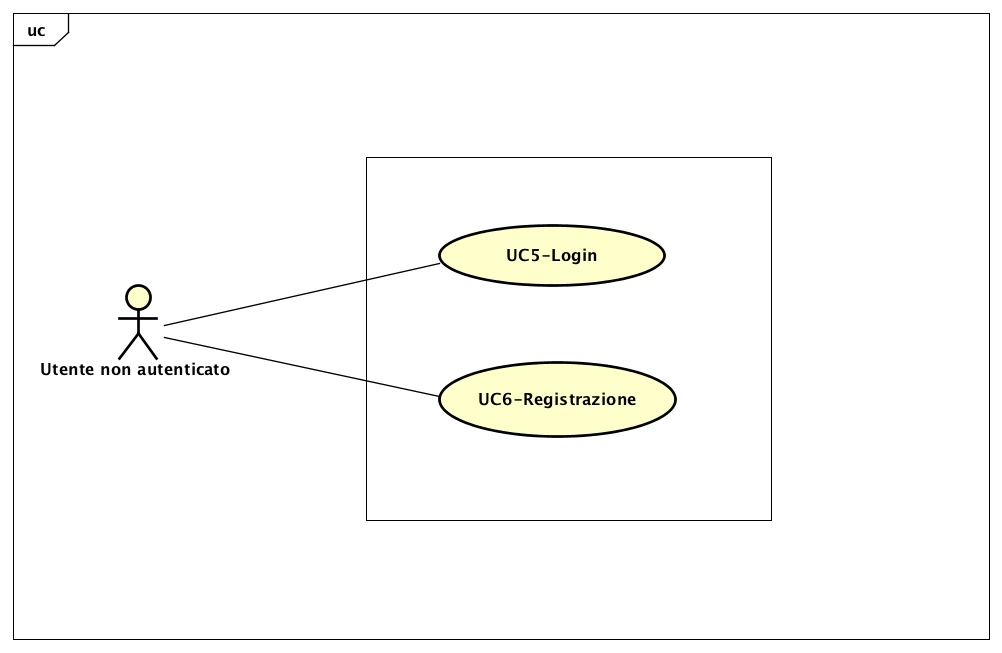
\includegraphics[scale=0.4]{Diagram/UC1.png}
	\caption{Scenario principale}\label{}
\end{figure}

\begin{itemize}
	\item \textbf{Attori primari}: Utente non autenticato;
	\item \textbf{Attori secondari}: Amazon;
	\item \textbf{Descrizione:} Un utente non autenticato può registrarsi al nostro servizio se non ha ancora un account o effettuare il login, nel caso fosse già registrato;
	\item \textbf{Precondizione:} L'applicazione è avviata e pronta all'uso;
	\item \textbf{Flusso principale degli eventi}:
	\begin{enumerate}
		\item L'utente ha la possibilità di: Registrazione (UC1.1);
		\item L'utente ha la possibilità di: Login (UC1.2).
	\end{enumerate}
	\item \textbf{Postcondizione}: L'applicazione ha ricevuto tutte le informazioni dell'utente non autenticato sulle operazioni che vuole eseguire.
\end{itemize}

\section{Caso d'uso UC1.1: Registrazione}
\begin{figure} [h]
	\centering
	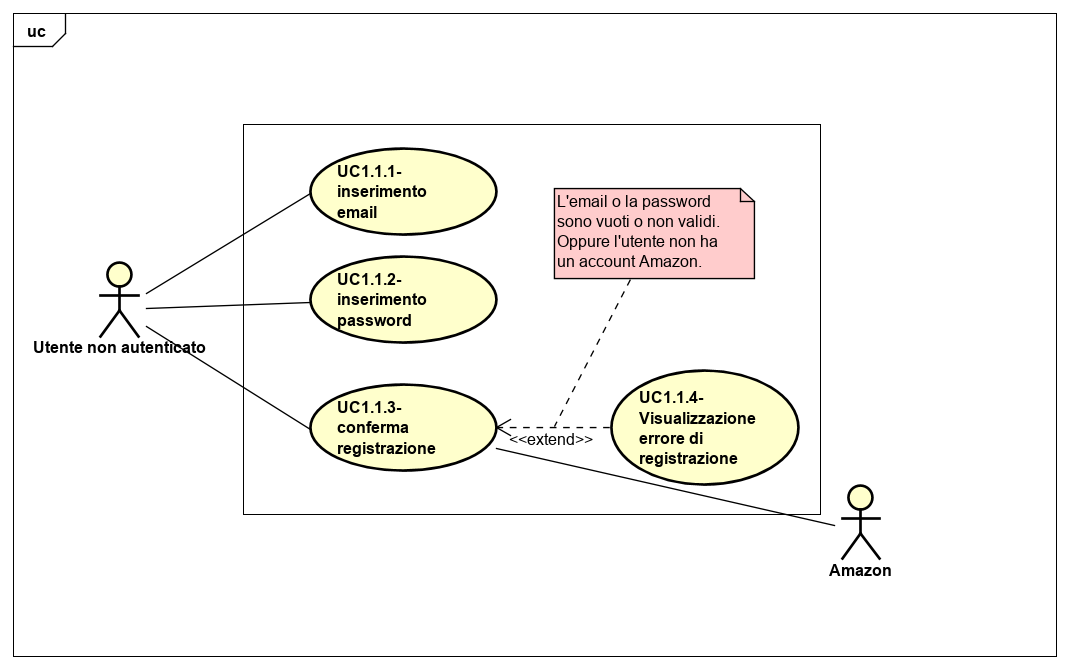
\includegraphics[scale=0.4]{./Diagram/UC1-1.png}
	\caption{Registrazione}\label{}
\end{figure}
\begin{itemize}
	\item \textbf{Attori primari}: Utente non autenticato;
	\item \textbf{Attori secondari}:\glossario{Amazon};
	\item \textbf{Descrizione}: Per accedere al sistema è necessario possedere un account;
	\item \textbf{Precondizione}: L'attore non possiede un account per accedere al sistema;
	\item \textbf{Flusso principale degli eventi}: 
	\begin{enumerate}
		\item L'attore inserisce la propria email (UC1.1.1);
		\item L'attore inserisce la propria password (UC1.1.2);
		\item L'attore conferma la registrazione(UC1.1.3).
	\end{enumerate}
	\item \textbf{Scenario alternativo}: L'attore dopo aver confermato le proprie credenziali visualizza un messaggio d'errore (UC1.1.4);
	\item \textbf{Postcondizione}:E' stato creato un account per accedere al sistema;
	\item \textbf{Estensioni}:
	\begin{enumerate}
		\item	Visualizzazione errore di registrazione(UC1.1.4).
	\end{enumerate}
\end{itemize}

\section{Caso d'uso UC1.1.1: Inserimento email}
\begin{itemize}
	\item \textbf{Attori primari}: Utente non autenticato;
	\item \textbf{Descrizione}: L'attore deve inserire la propria email per effettuare la  registrazione;
	\item \textbf{Precondizione}: Il sistema mostra il campo per l'inserimento della email;
	\item \textbf{Flusso principale degli eventi}: L'attore inserisce la propria email per effettuare la registrazione;
	\item \textbf{Postcondizione}: E' stata inserita l'email dell'attore nel campo opportuno.
\end{itemize}
\section{Caso d'uso UC1.1.2: Inserimento password}
\begin{itemize}
	\item \textbf{Attori primari}: Utente non autenticato;
	\item \textbf{Descrizione}: L'attore deve inserire la propria password per effettuare la registrazione;
	\item \textbf{Precondizione}: Il sistema mostra il campo per l'inserimento della password;
	\item \textbf{Flusso principale degli eventi}: L'attore inserisce la propria password per effettuare la registrazione;
	\item \textbf{Postcondizione}: È stata inserita la password dell'attore nel campo opportuno.
\end{itemize}

\section{Caso d'uso UC1.1.3: Conferma registrazione}
\begin{itemize}
	\item \textbf{Attori primari}: Utente non autenticato;
	\item \textbf{Descrizione}: L'attore dopo aver compilato i campi richiesti decide di confermare  la registrazione;
	\item \textbf{Precondizione}: Il sistema mostra un pulsante per confermare la registrazione;
	\item \textbf{Flusso principale degli eventi}:L'attore decide di confermare la registrazione per completarla;
	\item \textbf{Postcondizione:} Il sistema registra l'attore poiché questo ha confermato l'operazione;
	\item \textbf{Estensione:}
	\begin{itemize}
		\item Visualizzazione dell'errore di registrazione(UC1.1.4).
	\end{itemize}
\end{itemize}


\section{Caso d'uso UC1.1.4: Visualizzazione dell'errore di registrazione}
\begin{itemize}
	\item \textbf{Attori primari}: Utente non autenticato;
	\item \textbf{Descrizione}: L'attore visualizza un errore nel caso avesse compilato i campi con dati errati;
	\item \textbf{Precondizione}: Il sistema ha ricevuto campi dati errati: vuoti o non validi;
	\item \textbf{Flusso principale degli eventi}: L'attore visualizza il messaggio d'errore relativo al campo dato del:
	\begin{itemize}
		\item E-mail;
		\item Password.
	\end{itemize}
	\item \textbf{Postcondizione:} Il sistema mostra un messaggio d'errore per segnalare il tentativo di registrarsi con campi dati errati.
\end{itemize}

\section{Caso d'uso UC1.2: Login}
\begin{figure} [h]
	\centering
	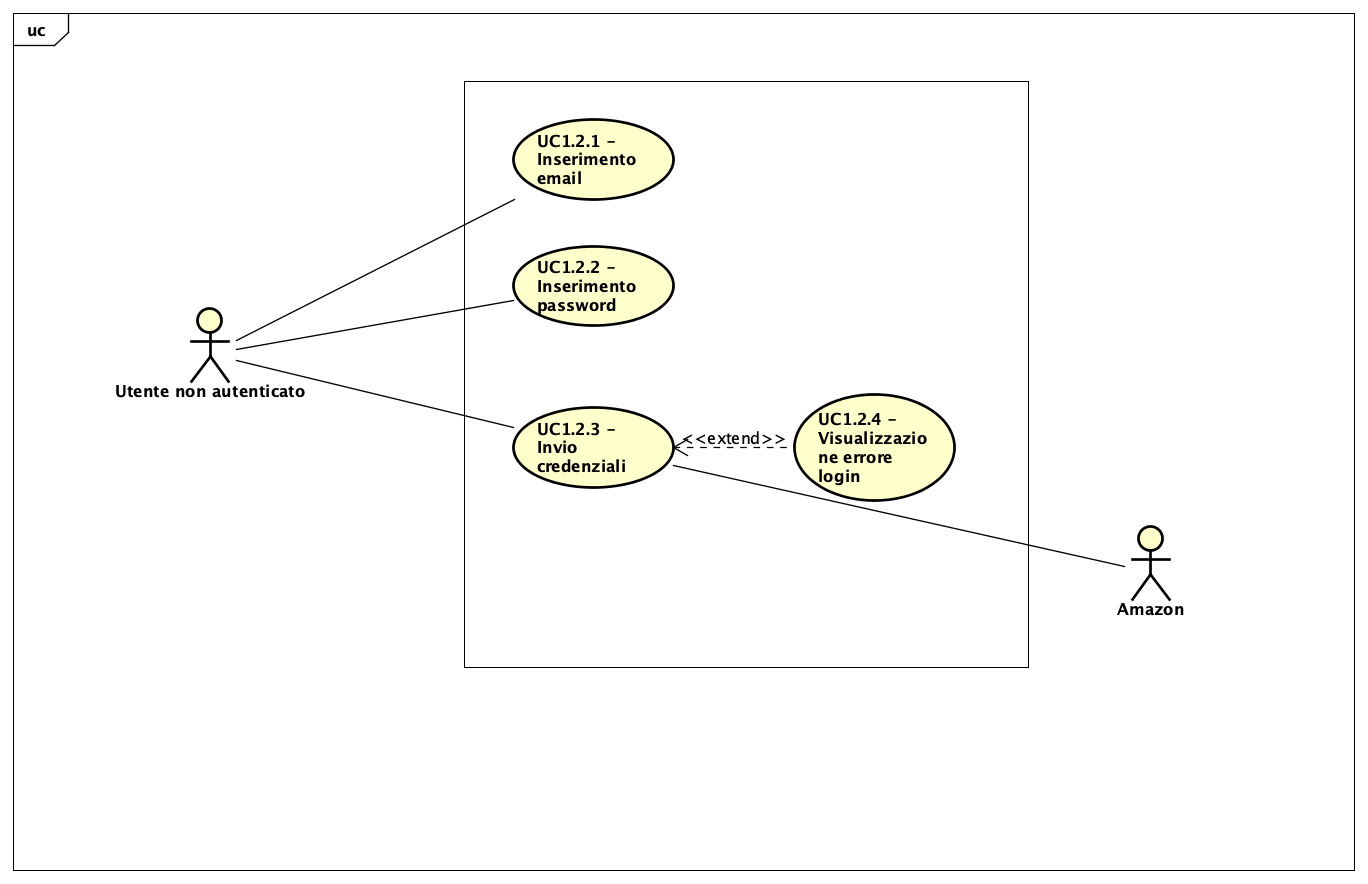
\includegraphics[scale=0.4]{./Diagram/UC1-2.png}
	\caption{Login}\label{}
\end{figure}
\begin{itemize}
	\item \textbf{Attori primari}: Utente non autenticato;
	\item \textbf{Attori secondari}:\glossario{Amazon};
	\item \textbf{Descrizione}: Il sistema è avviato, ma è necessario effettuare il login per accedervi;
	\item \textbf{Precondizione}: Il sistema non permette l'accesso all'utente non autenticato;
	\item \textbf{Flusso principale degli eventi}:
	\begin{enumerate}
		\item L'utente inserisce la propria email (UC1.2.1);
		\item L'utente inserisce la propria password (UC1.2.2);
		\item L'utente invia le credenziali (UC1.2.3).
	\end{enumerate}
	\item \textbf{Scenario alternativo}: L'utente dopo aver inviato le proprie credenziali visualizza un messaggio d'errore (UC1.2.4);
	\item \textbf{Postcondizione}: Il sistema permette l'accesso all'utente che ora diventa un utente autenticato; 
	\item \textbf{Generalizzazioni}:
	\begin{enumerate}
		\item Login automatico (UC1.3).
	\end{enumerate}
\end{itemize}


\section{Caso d'uso UC1.2.1: Inserimento email}
\begin{itemize}
	\item \textbf{Attori primari}: Utente non autenticato;
	\item \textbf{Descrizione}: L'utente inserisce la sua email per effettuare il login;
	\item \textbf{Precondizione}: Il sistema fa visualizzare il campo email;
	\item \textbf{Flusso principale degli eventi}: L'attore inserisce la sua mail per effettuare il login;
	\item \textbf{Postcondizione:} E' stata inserita la mail dell'attore nel campo predisposto. 
\end{itemize}

\section{Caso d'uso UC1.2.2: Inserimento password}
\begin{itemize}
	\item \textbf{Attori primari}: Utente non autenticato;
	\item \textbf{Descrizione}: L'utente inserisce la sua password per effettuare il login;
	\item \textbf{Precondizione}: Il sistema fa visualizzare il campo password;
	\item \textbf{Flusso principale degli eventi}: L'attore inserisce la sua password per effettuare il login;
	\item \textbf{Postcondizione:} E' stata inserita la password dell'attore nel campo predisposto. 
\end{itemize}
\section{Caso d'uso UC1.2.3: Invio credenziali}
\begin{itemize}
	\item \textbf{Attori primari}: Utente non autenticato;
	\item \textbf{Descrizione:} Dopo aver inserito tutti i dati l'utente conferma il login;
	\item \textbf{Precondizione}: Il sistema far visualizzare la pagina di login;
	\item \textbf{Flusso principale degli eventi}: L'attore dopo aver inserito le credenziali può confermare il login;
	\item \textbf{Postcondizione}: L'utente è riconosciuto dal sistema come utente autenticato;
	\item \textbf{Scenari alternativi}: L'utente inserisce credenziali errate e viene visualizzato un messaggio d'errore;
	\item \textbf{Estensioni}:
	\begin{enumerate}
		\item Visualizzazione errore login (UC1.2.4).
	\end{enumerate} 
\end{itemize}
\section{Caso d'uso UC1.2.4: Visualizzazione errore login}
\begin{itemize}
	\item \textbf{Attori primari}: Utente non autenticato;
	\item \textbf{Descrizione:} L'attore può aver inserito delle credenziali errate;
	\item \textbf{Precondizione}: Il sistema ha ricevuto campi dati errati;
	\item \textbf{Flusso principale degli eventi}: L'attore visualizza un messaggio d'errore;
	\item \textbf{Postcondizione:} L'utente non è riconosciuto dal sistema.
\end{itemize}
\section{Caso d'uso UC1.3: Login automatico}
\begin{itemize}
	\item \textbf{Attori primari}: Utente non autenticato;
	\item \textbf{Attori secondari}:\glossario{Amazon};
	\item \textbf{Descrizione}: Il sistema è avviato, ma è necessario effettuare il login per accedervi;
	\item \textbf{Precondizione}: Il sistema non permette l'accesso all'utente non autenticato;
	\item \textbf{Scenario alternativo}: L'utente dopo aver inviato le proprie credenziali visualizza un messaggio d'errore (UC1.2.4);
	\item \textbf{Postcondizione}: Il sistema permette l'accesso all'utente che ora diventa un utente autenticato.
\end{itemize}
\section{Caso d'uso UC2: Scenario principale dell'utente autenticato}
\begin{figure} [h]
	\centering
	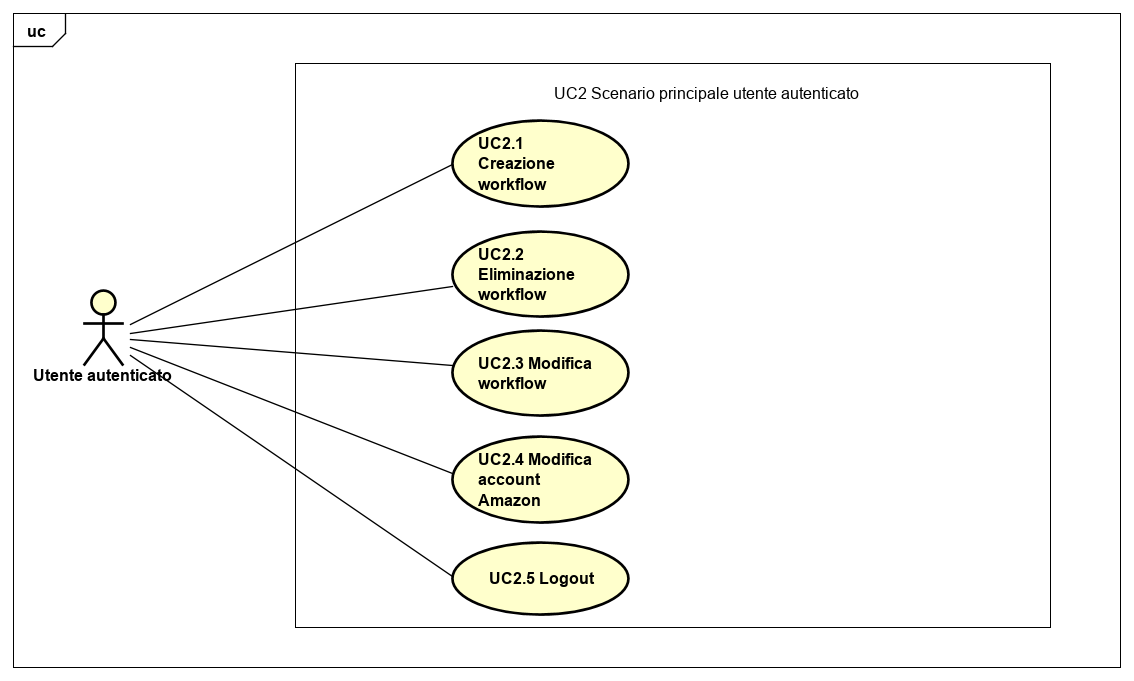
\includegraphics[scale=0.4]{./Diagram/UC2.png}
	\caption{Scenario principale dell'utente autenticato }\label{}
\end{figure}
\begin{itemize}
	\item \textbf{Attori primari}: Utente autenticato;
	\item \textbf{Descrizione:} L'attore può creare, modificare ed eliminare un\glossario{workflow}, modificare i propri dati personali ed eseguire il logout;
	\item \textbf{Precondizione:} Il sistema mostra la pagina principale per l'utente autenticato;
	\item \textbf{Flusso principale degli eventi:}
	\begin{enumerate}
		\item L'utente può creare un\glossario{workflow}(UC2.1);
		\item L'utente può eliminare un workflow (UC2.2);
		\item L'utente può modificare un workflow (UC2.3);
		\item L'utente può modificare l'account\glossario{Amazon}(UC2.4);
		\item L'utente può effettuare il Logout (UC2.5).
	\end{enumerate}
	\item \textbf{Postcondizione:} Il sistema ha ricevuto le informazioni riguardanti i comandi che l'utente vuole eseguire.
\end{itemize}
\section{Caso d'uso UC2.1: Creazione workflow}
\begin{figure} [h]
	\centering
	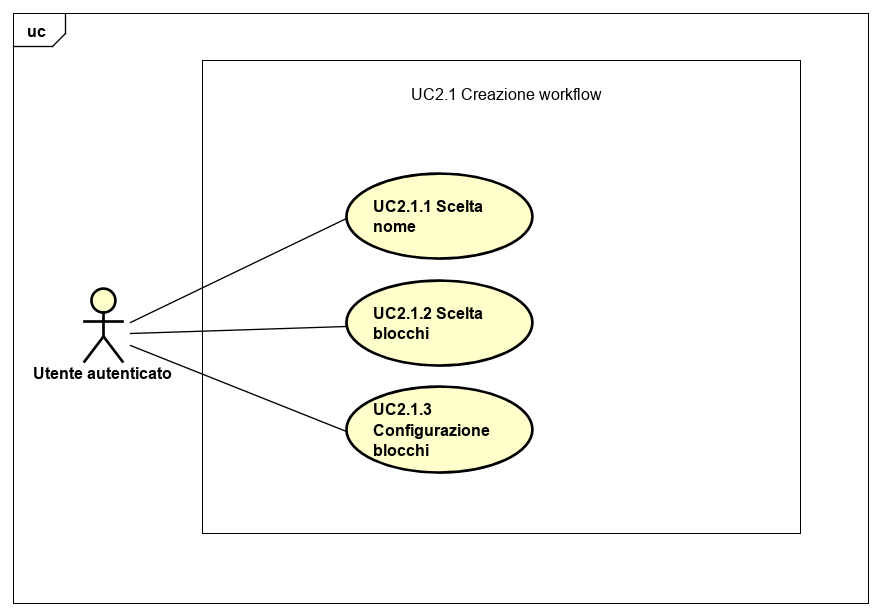
\includegraphics[scale=0.4]{./Diagram/UC2-1.png}
	\caption{Scenario principale dell'utente autenticato }\label{}
\end{figure}
\begin{itemize}
	\item \textbf{Attori primari}: Utente autenticato;
	\item \textbf{Descrizione:} L'attore può creare un\glossario{workflow}selezionando e configurando i blocchi disponibili;
	\item \textbf{Precondizione:} Il sistema mette a disposizione un form per la creazione di un \textit{workflow$_{G}$};
	\item \textbf{Flusso principale degli eventi:}
	\begin{enumerate}
		\item L'utente sceglie il nome del\glossario{workflow}(UC2.1.1);
		\item L'utente seleziona quali blocchi vuole usare (UC2.1.2);
		\item L'utente configura i blocchi selezionati (UC2.1.3).
	\end{enumerate}
	\item \textbf{Postcondizione:} Il sistema contiene il workflow desiderato dall'attore.
\end{itemize}
\section{Caso d'uso UC2.1.1: Scelta nome }
\begin{itemize}
	\item \textbf{Attori primari}: Utente autenticato;
	\item \textbf{Descrizione:} L'attore inserisce il nome del \textit{workflow$_{G}$};
	\item \textbf{Precondizione:} Il sistema mette a disposizione un campo per l'inserimento del nome;
	\item \textbf{Flusso principale degli eventi:}
	\begin{enumerate}
		\item L'utente inserisce il nome del workflow.
	\end{enumerate}
	\item \textbf{Postcondizione:} Il form di creazione del workflow contiene il nome del workflow.
\end{itemize}
\section{Caso d'uso UC2.1.2: Scelta blocchi }
\begin{itemize}
	\item \textbf{Attori primari}: Utente autenticato;
	\item \textbf{Descrizione:} L'attore sceglie i blocchi che compongono il \textit{workflow$_{G}$};
	\item \textbf{Precondizione:} Il sistema mette a disposizione un form per l'inserimento dei blocchi e una lista di blocchi disponibili;
	\item \textbf{Flusso principale degli eventi:}
	\begin{enumerate}
		\item L'attore inserisce i blocchi nel form e li ordina come preferisce.
	\end{enumerate}
	\item \textbf{Postcondizione:} Il workflow contiene i blocchi desiderati dall'utente.
\end{itemize}
\section{Caso d'uso UC2.1.3: Configurazione blocchi }
\begin{itemize}
	\item \textbf{Attori primari}: Utente autenticato;
	\item \textbf{Descrizione:} L'attore configura i blocchi che compongono il \textit{workflow$_{G}$};
	\item \textbf{Precondizione:} Il sistema mette a disposizione un form per la configurazione dei blocchi;
	\item \textbf{Flusso principale degli eventi:}
	\begin{enumerate}
		\item L'attore configura i blocchi.
	\end{enumerate}
	\item \textbf{Postcondizione:} Il workflow contiene solo blocchi configurati.
\end{itemize}
\section{Caso d'uso UC2.2: Eliminazione workflow}
\begin{itemize}
	\item \textbf{Attori primari}: Utente autenticato;
	\item \textbf{Descrizione:} L'attore elimina un \textit{workflow$_{G}$};
	\item \textbf{Precondizione:} Il sistema mette a disposizione un comando per eliminare un workflow;
	\item \textbf{Flusso principale degli eventi:}
	\begin{enumerate}
		\item L'utente seleziona il comando per eliminare workflow che vuole rimuovere.
	\end{enumerate}
	\item \textbf{Postcondizione:} Il\glossario{workflow}che l'attore voleva eliminare è stato rimosso dal sistema.
\end{itemize}
\section{Caso d'uso UC2.3: Modifica workflow}
\begin{figure} [h]
	\centering
	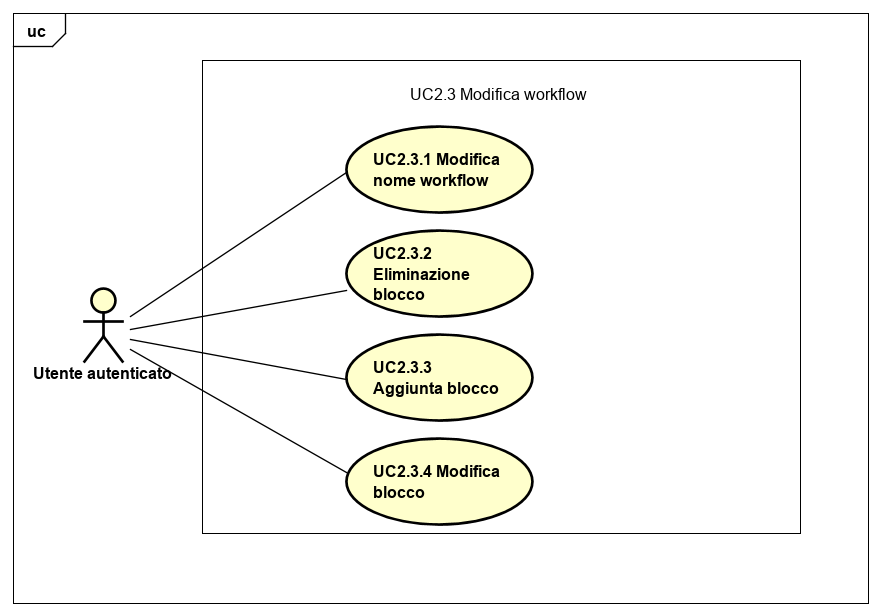
\includegraphics[scale=0.4]{./Diagram/UC2-3.png}
	\caption{Modifica workflow }\label{}
\end{figure}
\begin{itemize}
	\item \textbf{Attori primari}: Utente autenticato;
	\item \textbf{Descrizione:} L'attore modifica un \textit{workflow$_{G}$};
	\item \textbf{Precondizione:} Il sistema mette a disposizione un form per la modifica di un workflow;
	\item \textbf{Flusso principale degli eventi:}
	\begin{enumerate}
		\item L'attore può cambiare il nome del\glossario{workflow}(UC2.3.1);
		\item L'attore può eliminare un blocco dal workflow (UC2.3.2);
		\item L'attore può aggiungere un blocco nel workflow (UC2.3.3);
		\item L'attore può modificare la configurazione di un blocco presente nel workflow (UC2.3.4).
	\end{enumerate}
	\item \textbf{Postcondizione:} Il\glossario{workflow}è stato modificato.
\end{itemize}
\section{Caso d'uso UC2.3.1: Modifica nome workflow}
\begin{itemize}
	\item \textbf{Attori primari}: Utente autenticato;
	\item \textbf{Descrizione:} L'attore modifica il nome del \textit{workflow$_{G}$};
	\item \textbf{Precondizione:} Il sistema mette a disposizione un campo per l'inserimento del nuovo nome;
	\item \textbf{Flusso principale degli eventi:}
	\begin{enumerate}
		\item L'attore inserisce il nuovo nome del workflow.
	\end{enumerate}
	\item \textbf{Postcondizione:} Il form di creazione del workflow contiene il nuovo nome del workflow.
\end{itemize}
\section{Caso d'uso UC2.3.2: Eliminazione blocco }
\begin{itemize}
	\item \textbf{Attori primari}: Utente autenticato.
	\item \textbf{Descrizione:} L'attore rimuove il blocco che non desidera più dal \textit{workflow$_{G}$};
	\item \textbf{Precondizione:} Il sistema fornisce un comando per l'eliminazione del blocco;
	\item \textbf{Flusso principale degli eventi:}
	\begin{enumerate}
		\item L'attore elimina il blocco.
	\end{enumerate}
	\item \textbf{Postcondizione:} Il workflow non contiene più il blocco indesiderato dall'attore.
\end{itemize}
\section{Caso d'uso UC2.3.3: Aggiunta blocco }
\begin{itemize}
	\item \textbf{Attori primari}: Utente autenticato;
	\item \textbf{Descrizione:} L'attore aggiunge il nuovo blocco al \textit{workflow$_{G}$};
	\item \textbf{Precondizione:} Il sistema mette a disposizione un form per l'aggiunta del blocco;
	\item \textbf{Flusso principale degli eventi:}
	\begin{enumerate}
		\item L'attore aggiunge il blocco;
		\item L'attore configura il nuovo blocco.
	\end{enumerate}
	\item \textbf{Postcondizione:} Il workflow contiene il nuovo blocco configurato.
\end{itemize}
\section{Caso d'uso UC2.3.4: Modifica blocco }
\begin{itemize}
	\item \textbf{Attori primari}: Utente autenticato;
	\item \textbf{Descrizione:} L'attore modifica la configurazione del blocco che compone il \textit{workflow$_{G}$};
	\item \textbf{Precondizione:} Il sistema mette a disposizione un form per la modifica dei blocchi;
	\item \textbf{Flusso principale degli eventi:}
	\begin{enumerate}
		\item L'attore modifica la configurazione del blocco.
	\end{enumerate}
	\item \textbf{Postcondizione:} Il blocco desiderato dall'attore è stato riconfigurato.
\end{itemize}
\section{Caso d'uso UC2.4: Modifica account Amazon }
\begin{itemize}
	\item \textbf{Attori primari}: Utente autenticato;
	\item \textbf{Descrizione:} L'attore cambia il proprio account \textit{Amazon$_{G}$};
	\item \textbf{Precondizione:} Il sistema mette a disposizione un form per la modifica dell'account Amazon.
	\item \textbf{Flusso principale degli eventi:}
	\begin{enumerate}
		\item L'attore, attraverso il form di Amazon, sceglie il nuovo account.
	\end{enumerate}
	\item \textbf{Postcondizione:} Il sistema è collegato al nuovo account Amazon.
	\item \textbf{Estensione:}
	\begin{itemize}
		\item Visualizzazione dell'errore di cambio Account (UC2.4.1);
	\end{itemize}
\end{itemize}
\section{Caso d'uso UC2.4.1: Errore di cambio account Amazon }
\begin{itemize}
	\item \textbf{Attori primari}: Utente autenticato;
	\item \textbf{Descrizione:} L'attore ha inserito dei dati non corretti e non riesce a collegarsi al nuovo account \textit{Amazon$_{G}$};
	\item \textbf{Precondizione:} Il sistema non riesce a collegarsi all'account Amazon;
	\item \textbf{Flusso principale degli eventi:}
	\begin{enumerate}
		\item L'attore può inserire nuovamente i dati nel form di Amazon;
		\item L'attore può tornare al vecchio account Amazon.
	\end{enumerate}
	\item \textbf{Postcondizione:} Il sistema è correttamente collegato a un account Amazon.
\end{itemize}
\section{Caso d'uso UC2.5: Logout }
\begin{itemize}
	\item \textbf{Attori primari}: Utente autenticato;
	\item \textbf{Descrizione:} L'attore effettua il logout dall'applicazione;
	\item \textbf{Precondizione:} Il sistema fornisce un metodo per permettere all'utente di disconnettersi dal sistema;
	\item \textbf{Flusso principale degli eventi:}
	\begin{enumerate}
		\item L'attore si disconnette dal sistema.
	\end{enumerate}
	\item \textbf{Postcondizione:} Il sistema non riconosce più l'utente.
\end{itemize}

	\chapter{Requisiti} \label{Requisiti}
Vengono riportati i\glossario{requisiti}individuati basandosi sui casi d'uso, sul \textit{capitolato$_{G}$}, sui diversi incontri avuti con l'azienda \textit{Zero12 s.r.l.} e per necessità interne. \\

Ogni\glossario{requisito}deve avere la seguente nomenclatura:
\begin{center}
	\textbf{R$\Bigl\{$A$\Bigr\}$$\Bigl\{$B$\Bigr\}$$\Bigl\{$XX$\Bigr\}$.$\Bigl\{$YY$\Bigr\}$}
\end{center}
dove:
\begin{itemize}
	\item \textbf{A:} corrisponde a uno dei seguenti requisiti:
	\begin{itemize}
		\item F: funzionale;
		\item Q: di qualità;
		\item P: di prestazione;
		\item V: di vincolo.
	\end{itemize}
	\item \textbf{B:} corrisponde a uno dei seguenti requisiti:
	\begin{itemize}
		\item O: obbligatorio;
		\item F: facoltativo;
		\item D: desiderabile.
	\end{itemize}
	\item \textbf{{XX}:} numero che identifica i\glossario{requisiti};
	\item \textbf{{YY}:} numero progressivo che identifica i sottocasi, esso può, a sua volta, includere altri sottocasi.
\end{itemize}
\pagebreak
\section{Requisiti Funzionali}
\normalsize
\begin{longtable}{|c|>{\centering}m{7cm}|c|}
	\hline 
	\textbf{Id Requisito} & \textbf{Descrizione} & \textbf{Stato}\\
	\hline
	\endhead
	\hypertarget{RFO1}{RFO1} & L'applicazione deve permettere all'utente non autenticato di registrarsi con un account Amazon & \textit{Non Soddisfatto}\\ \hline
	
	\hypertarget{RFO2}{RFO2} & L'applicazione deve permettere all'utente non autenticato di effettuare il login automatico con l'account Amazon & \textit{Non Soddisfatto}\\ \hline
	
	\hypertarget{RFO3}{RFO3} & L'applicazione deve permettere all'utente non autenticato di effettuare il login manuale con l'account Amazon & \textit{Non Soddisfatto}\\ \hline
	
	\hypertarget{RFO4}{RFO4} & L'applicazione deve permettere all'utente autenticato di effettuare il logout & \textit{Non Soddisfatto}\\ \hline
	
	\hypertarget{RFO5}{RFO5} & L'applicazione deve permettere all'utente autenticato di modificare l'account Amazon & \textit{Non Soddisfatto}\\ \hline
	
	\hypertarget{RFO6}{RFO6} & L'utente tramite Alexa deve poter impostare una sveglia & \textit{Non Soddisfatto}\\ \hline
	
	\hypertarget{RFO6.1}{RFO6.1} & L'utente tramite Alexa deve poter creare una nuova sveglia & \textit{Non Soddisfatto}\\ \hline
	
	\hypertarget{RFO6.2}{RFO6.2} & L'utente tramite Alexa deve poter modificare l'orario di una sveglia & \textit{Non Soddisfatto}\\ \hline
	
	\hypertarget{RFO6.3}{RFO6.3} & L'utente tramite Alexa deve poter posporre una sveglia mentre questa sta suonando & \textit{Non Soddisfatto}\\ \hline
	
	\hypertarget{RFO6.4}{RFO6.4} & L'utente tramite Alexa deve poter interrompere una sveglia mentre questa sta suonando & \textit{Non Soddisfatto}\\ \hline
	
	\hypertarget{RFO7}{RFO7} & L'utente tramite Alexa deve poter inserire un Pin per proteggere il workflow & \textit{Non Soddisfatto}\\ \hline
	
	\hypertarget{RFO8}{RFO8} & L'utente tramite Alexa deve poter gestire una lista & \textit{Non Soddisfatto}\\ \hline
	
	\hypertarget{RFO9}{RFO9} & L'utente tramite Alexa deve poter ascoltare i tweet & \textit{Non Soddisfatto}\\ \hline
	
	\hypertarget{RFO10}{RFO10} & L'utente tramite Alexa deve poter inviare delle mail & \textit{Non Soddisfatto}\\ \hline
	
	\hypertarget{RFO11}{RFO11} & L'utente tramite Alexa deve poter leggere le proprie mail & \textit{Non Soddisfatto}\\ \hline
	
	\hypertarget{RFO12}{RFO12} & Alexa deve essere in grado di riprodurre un blocco di testo personalizzato & \textit{Non Soddisfatto}\\ \hline
	
	\hypertarget{RFO13}{RFO13} & L'utente potrà ascoltare gli eventi presenti nel proprio calendario personale tramite Alexa & \textit{Non Soddisfatto}\\ \hline
	
	\hypertarget{RFO14}{RFO14} & L'utente potrà inserire eventi in programma nel proprio calendario personale tramite Alexa & \textit{Non Soddisfatto}\\ \hline
	
	\hypertarget{RFO15}{RFO15} & L'applicazione deve permettere all'utente autenticato la creazione di un workflow & \textit{Non Soddisfatto}\\ \hline
	
	\hypertarget{RFO15.1}{RFO15.1} & L'applicazione deve permettere all'utente autenticato di inserire il nome del workflow & \textit{Non Soddisfatto}\\ \hline
	
	\hypertarget{RFO15.2}{RFO15.2} & L'applicazione deve permettere all'utente autenticato di aggiungere un blocco & \textit{Non Soddisfatto}\\ \hline
	
	\hypertarget{RFO16}{RFO16} & L'applicazione deve permettere all'utente autenticato di eliminare un workflow & \textit{Non Soddisfatto}\\ \hline
	
	\hypertarget{RFO17}{RFO17} & L'applicazione deve permettere all'utente autenticato di modificare un workflow & \textit{Non Soddisfatto}\\ \hline
	
	\hypertarget{RFO17.1}{RFO17.1} & L'applicazione deve permettere all'utente autenticato di cambiare il nome di un workflow & \textit{Non Soddisfatto}\\ \hline
	
	\hypertarget{RFO17.2}{RFO17.2} & L'applicazione deve permettere all'utente autenticato di modificare i blocchi contenuti in un workflow & \textit{Non Soddisfatto}\\ \hline
	
	\hypertarget{RFO18}{RFO18} & L'utente tramite Alexa deve poter ascoltare il risultato prodotto dal feed RSS & \textit{Non Soddisfatto}\\ \hline
	
	\hypertarget{RFO19}{RFO19} & L'utente potrà ascoltare news da un sito di notizie tramite Alexa & \textit{Non Soddisfatto}\\ \hline
	
	\hypertarget{RFO20}{RFO20} & L'utente potrà ascoltare notizie sportive tramite Alexa & \textit{Non Soddisfatto}\\ \hline
	
	\hypertarget{RFO21}{RFO21} & L'utente potrà applicare un filtro sul numero di risultati ricevuti in output da Alexa & \textit{Non Soddisfatto}\\ \hline
	
	\hypertarget{RFO22}{RFO22} & L'utente potrà ricevere informazioni sul meteo tramite Alexa & \textit{Non Soddisfatto}\\ \hline
	
	\hypertarget{RFO23}{RFO23} & L'utente potrà predisporre il suo workflow personalizzato per la riproduzione di musica con Amazon Music tramite Alexa & \textit{Non Soddisfatto}\\ \hline
	
	\hypertarget{RFO24}{RFO24} & L'utente tramite Alexa deve poter mettere in pausa un workflow & \textit{Non Soddisfatto}\\ \hline
	
	\hypertarget{RFO25}{RFO25} & Alexa deve fornire un sistema di aiuto che dice all'utente in qualsiasi istante in quale punto dell'esecuzione si trova & \textit{Non Soddisfatto}\\ \hline
	
	\hypertarget{RFF26}{RFF26} & I dati utente verranno automaticamente sincronizzati con il proprio account Amazon & \textit{Non Soddisfatto}\\ \hline
	
	\hypertarget{RFF27}{RFF27} & L'utente deve poter rispondere ad un tweet dopo che Alexa l'ha letto & \textit{Non Soddisfatto}\\ \hline
	
	\hypertarget{RFF28}{RFF28} & L'utente deve poter rispondere ad una mail dopo che Alexa l'ha letta & \textit{Non Soddisfatto}\\ \hline
	
	\hypertarget{RFF29}{RFF29} & L'utente deve poter inviare messaggi di testo su Telegram tramite Alexa a una persona o ad un gruppo & \textit{Non Soddisfatto}\\ \hline
	
	\hypertarget{RFF30}{RFF30} &  L'utente deve poter leggere tramite Alexa i nuovi messaggi testuali ricevuti da una persona o un gruppo su Telegram & \textit{Non Soddisfatto}\\ \hline
	
	\hypertarget{RFF31}{RFF31} & L'utente deve poter inviare messaggi audio su Telegram tramite Alexa a una persona o un gruppo & \textit{Non Soddisfatto}\\ \hline
	
	\hypertarget{RFF32}{RFF32} & L'utente deve poter modificare un evento nel calendario tramite Alexa & \textit{Non Soddisfatto}\\ \hline
	
	\hypertarget{RFF33}{RFF33} & L'utente potrà predisporre il suo workflow personalizzato per la riproduzione di musica tramite Youtube & \textit{Non Soddisfatto}\\ \hline
	
	\hypertarget{RFF34}{RFF34} & L'utente tramite Alexa può impostare un timer & \textit{Non Soddisfatto}\\ \hline
	
	\hypertarget{RFF35}{RFF35} & L'utente tramite Alexa può ascoltare la radio & \textit{Non Soddisfatto}\\ \hline
	
	\hypertarget{RFF36}{RFF36} & L'utente tramite Alexa può controllare l'illuminazione, se compatibile con il dispositivo & \textit{Non Soddisfatto}\\ \hline
	
	\hypertarget{RFF36.1}{RFF36.1} & L'utente tramite Alexa può accendere le luci & \textit{Non Soddisfatto}\\ \hline
	
	\hypertarget{RFF36.2}{RFF36.2} & L'utente tramite Alexa può spegnere le luci & \textit{Non Soddisfatto}\\ \hline
	
	\hypertarget{RFD37}{RFD37} & L'utente tramite Alexa può pubblicare un tweet all'interno di Twitter & \textit{Non Soddisfatto}\\ \hline
	
	\hypertarget{RFD38}{RFD38} & L'utente tramite Alexa può ascoltare la musica tramite il servizio di Spotify & \textit{Non Soddisfatto}\\ \hline
	
	\hypertarget{RFD39}{RFD39} & L'utente tramite Alexa può utilizzare un blocco per la pianificazione dell'apertura di un altro blocco in automatico & \textit{Non Soddisfatto}\\ \hline
	
	\hypertarget{RFD40}{RFD40} & L'utente tramite Alexa può ascoltare le notizie riguardanti la borsa e le criptovalute & \textit{Non Soddisfatto}\\ \hline
	
	\caption[Requisiti Funzionali]{Requisiti Funzionali}
	\label{tabella:req0}
\end{longtable}
\clearpage
\section{Requisiti Prestazionali}
\normalsize
\begin{longtable}{|c|>{\centering}m{7cm}|c|}
	\hline 
	\textbf{Id Requisito} & \textbf{Descrizione} & \textbf{Stato}\\
	\hline
	\endhead
	\hypertarget{RPO1}{RPO1} & L'applicazione Android deve essere compatibile dalla versione 4.4 & \textit{Non Soddisfatto}\\ \hline
	
	\caption[Requisiti Prestazionali]{Requisiti Prestazionali}
	\label{tabella:req1}
\end{longtable}
\clearpage
\section{Requisiti di Qualità}
\normalsize
\begin{longtable}{|c|>{\centering}m{7cm}|c|}
	\hline 
	\textbf{Id Requisito} & \textbf{Descrizione} & \textbf{Stato}\\
	\hline
	\endhead
	\hypertarget{RQO1}{RQO1} & Deve essere fornita la documentazione dettagliata di tutte le API & \textit{Non Soddisfatto}\\ \hline
	
	\hypertarget{RQO2}{RQO2} & Devono essere forniti i diagrammi UML relativi agli Use Cases di progetto & \textit{Non Soddisfatto}\\ \hline
	
	\hypertarget{RQO3}{RQO3} & Devono essere forniti i Voice Dialog Flow & \textit{Non Soddisfatto}\\ \hline
	
	\hypertarget{RQO4}{RQO4} & Deve essere fornito lo Schema Design relativo alla base dati & \textit{Non Soddisfatto}\\ \hline
	
	\hypertarget{RQO5}{RQO5} & Deve essere fornito il \textit{Piano di test di unità} & \textit{Non Soddisfatto}\\ \hline
	
	\hypertarget{RQO6}{RQO6} & Deve essere consegnato il Bug Reporting per il tracciamento di tutte le problematiche o anomalie del sistema & \textit{Non Soddisfatto}\\ \hline
	
	\hypertarget{RQO7}{RQO7} & Tutta la documentazione prodotta in italiano dal team deve avere un indice di Gulpease compreso tra 60 e 100 & \textit{Non Soddisfatto}\\ \hline
	
	\hypertarget{RQO8}{RQO8} & Tutta la documentazione rispetta le \textit{Norme di Progetto v2.0.0} e le metriche del \textit{Piano di Qualifica v2.0.0} & \textit{Non Soddisfatto}\\ \hline
	
	\hypertarget{RQO9}{RQO9} & Il codice prodotto rispetta le \textit{Norme di Progetto v2.0.0} e le metriche del \textit{Piano di Qualifica v2.0.0} & \textit{Non Soddisfatto}\\ \hline
	
	\caption[Requisiti di Qualità]{Requisiti di Qualità}
	\label{tabella:req2}
\end{longtable}
\clearpage
\section{Requisiti di Vincolo}
\normalsize
\begin{longtable}{|c|>{\centering}m{7cm}|c|}
	\hline 
	\textbf{Id Requisito} & \textbf{Descrizione} & \textbf{Stato}\\
	\hline
	\endhead
	\hypertarget{RVO1}{RVO1} & L'applicazione sarà utilizzabile da dispositivi Android & \textit{Non Soddisfatto}\\ \hline
	
	\hypertarget{RVO2}{RVO2} & L'applicazione deve essere sviluppata utilizzando il linguaggio di programmazione Kotlin & \textit{Non Soddisfatto}\\ \hline
	
	\hypertarget{RVO3}{RVO3} & Per lo sviluppo in back-end si utilizza NodeJS versione 10.15.1 & \textit{Non Soddisfatto}\\ \hline
	
	\hypertarget{RVO4}{RVO4} & Per i test viene utilizzato il framework Jasmine versione 3.3.0 & \textit{Non Soddisfatto}\\ \hline
	
	\hypertarget{RVO5}{RVO5} & Viene utilizzato il framework Express versione 4.16.4 per NodeJS & \textit{Non Soddisfatto}\\ \hline
	
	\hypertarget{RVO6}{RVO6} & Viene utilizzato DynamoDB come database NoSQL offerto dai servizi Amazon Web Services & \textit{Non Soddisfatto}\\ \hline
	
	\hypertarget{RVO7}{RVO7} & Si utilizza AWS Lambda per l'esecuzione del codice nel server & \textit{Non Soddisfatto}\\ \hline
	
	\hypertarget{RVO8}{RVO8} & Viene utilizzato NPM versione 6.4.1 per la gestione della build del codice prodotto & \textit{Non Soddisfatto}\\ \hline
	
	\caption[Requisiti di Vincolo]{Requisiti di Vincolo}
	\label{tabella:req3}
\end{longtable}
\clearpage

\section{Tracciamento Requisiti-Fonti}
\normalsize
\begin{longtable}{|>{\centering}m{5cm}|m{5cm}<{\centering}|}
	\hline
	\textbf{Id Requisito} & \textbf{Fonti}\\
	\hline
	\endhead
	\hyperlink{RFO1}{RFO1} & \hyperref[UC1.1]{UC1.1}\\ \hline
	
	\hyperlink{RFO2}{RFO2} & \hyperref[UC1.3]{UC1.3}\\ \hline
	
	\hyperlink{RFO3}{RFO3} & \hyperref[UC1.2]{UC1.2}\\ \hline
	
	\hyperlink{RFO4}{RFO4} & \hyperref[UC2.5]{UC2.5}\\ \hline
	
	\hyperlink{RFO5}{RFO5} & \hyperref[UC2.4]{UC2.4}\\ \hline
	
	\hyperlink{RFO6}{RFO6} & \hyperref[UC2.1.2.6]{UC2.1.2.6}\\ \hline
	
	\hyperlink{RFO6.1}{RFO6.1} & \hyperref[UC2.1.2.6]{UC2.1.2.6}\\ \hline
	
	\hyperlink{RFO6.2}{RFO6.2} & \hyperref[UC2.1.2.6]{UC2.1.2.6}\\ \hline
	
	\hyperlink{RFO6.3}{RFO6.3} & \hyperref[UC2.1.2.6]{UC2.1.2.6}\\ \hline
	
	\hyperlink{RFO6.4}{RFO6.4} & \hyperref[UC2.1.2.6]{UC2.1.2.6}\\ \hline
	
	\hyperlink{RFO7}{RFO7} & \hyperref[UC2.1.2.1]{UC2.1.2.1}\\ \hline
	
	\hyperlink{RFO8}{RFO8} & \hyperref[UC2.1.2.5]{UC2.1.2.5}\\ \hline
	
	\hyperlink{RFO9}{RFO9} & \hyperref[UC2.1.2.4]{UC2.1.2.4} \\& Verbale Esterno 2018-12-05\\ \hline
	
	\hyperlink{RFO10}{RFO10} & \hyperref[UC2.1.2.7]{UC2.1.2.7} \\& Verbale Esterno 2018-12-05\\ \hline
	
	\hyperlink{RFO11}{RFO11} & \hyperref[UC2.1.2.7]{UC2.1.2.7} \\& Verbale Esterno 2018-12-05\\ \hline
	
	\hyperlink{RFO12}{RFO12} & \hyperref[UC2.1.2.3]{UC2.1.2.3} \\& Verbale Esterno 2018-12-05\\ \hline
	
	\hyperlink{RFO13}{RFO13} & \hyperref[UC2.1.2.9]{UC2.1.2.9} \\& Verbale Esterno 2018-12-05\\ \hline
	
	\hyperlink{RFO14}{RFO14} & \hyperref[UC2.1.2.9]{UC2.1.2.9} \\& Verbale Esterno 2018-12-05\\ \hline
	
	\hyperlink{RFO15}{RFO15} & \hyperref[UC2.1]{UC2.1} \\& Verbale Esterno 2018-12-05\\ \hline
	\pagebreak
	\hyperlink{RFO15.1}{RFO15.1} & \hyperref[UC2.1.1]{UC2.1.1} \\& Verbale Esterno 2018-12-05\\ \hline
	
	\hyperlink{RFO15.2}{RFO15.2} & \hyperref[UC2.1.2]{UC2.1.2} \\& Verbale Esterno 2018-12-05\\ \hline
	
	\hyperlink{RFO16}{RFO16} & \hyperref[UC2.2]{UC2.2} \\& Verbale Esterno 2018-12-05\\ \hline
	
	\hyperlink{RFO17}{RFO17} & \hyperref[UC2.3]{UC2.3} \\& Verbale Esterno 2018-12-05\\ \hline
	
	\hyperlink{RFO17.1}{RFO17.1} & \hyperref[UC2.3.1]{UC2.3.1} \\& Verbale Esterno 2018-12-05\\ \hline
	
	\hyperlink{RFO17.2}{RFO17.2} & \hyperref[UC2.3.4]{UC2.3.4} \\& Verbale Esterno 2018-12-05\\ \hline
	
	\hyperlink{RFO18}{RFO18} & \hyperref[UC2.1.2.16]{UC2.1.2.16} \\& Verbale Esterno 2018-12-05\\ \hline
	
	\hyperlink{RFO19}{RFO19} & \hyperref[UC2.1.2.16]{UC2.1.2.16} \\& Verbale Esterno 2018-12-05\\ \hline
	
	\hyperlink{RFO20}{RFO20} & \hyperref[UC2.1.2.16]{UC2.1.2.16} \\& Verbale Esterno 2018-12-05\\ \hline
	
	\hyperlink{RFO21}{RFO21} & \hyperref[UC2.1.2.17]{UC2.1.2.17} \\& Verbale Esterno 2018-12-05\\ \hline
	
	\hyperlink{RFO22}{RFO22} & \hyperref[UC2.1.2.18]{UC2.1.2.18} \\& Verbale Esterno 2018-12-05\\ \hline
	
	\hyperlink{RFO23}{RFO23} & \hyperref[UC2.1.2.19]{UC2.1.2.19} \\& Verbale Esterno 2018-12-05\\ \hline
	
	\hyperlink{RFO24}{RFO24} & \hyperref[Interno]{Interno}\\ \hline
	
	\hyperlink{RFO25}{RFO25} & \hyperref[Interno]{Interno}\\ \hline
	
	\hyperlink{RFF26}{RFF26} & \hyperref[Interno]{Interno}\\ \hline
	
	\hyperlink{RFF27}{RFF27} & \hyperref[UC2.1.2.4]{UC2.1.2.4}\\ \hline
	
	\hyperlink{RFF28}{RFF28} & \hyperref[UC2.1.2.7]{UC2.1.2.7}\\ \hline
	
	\hyperlink{RFF29}{RFF29} & \hyperref[UC2.1.2.8]{UC2.1.2.8}\\ \hline
	
	\hyperlink{RFF30}{RFF30} & \hyperref[UC2.1.2.8]{UC2.1.2.8}\\ \hline
	
	\hyperlink{RFF31}{RFF31} & \hyperref[UC2.1.2.8]{UC2.1.2.8}\\ \hline
	
	\hyperlink{RFF32}{RFF32} & \hyperref[UC2.1.2.9]{UC2.1.2.9}\\ \hline
	
	\hyperlink{RFF33}{RFF33} & \hyperref[UC2.1.2.10]{UC2.1.2.10}\\ \hline
	
	\hyperlink{RFF34}{RFF34} & \hyperref[UC2.1.2.11]{UC2.1.2.11}\\ \hline
	
	\hyperlink{RFF35}{RFF35} & \hyperref[UC2.1.2.12]{UC2.1.2.12}\\ \hline
	
	\hyperlink{RFF36}{RFF36} & \hyperref[UC2.1.2.13]{UC2.1.2.13}\\ \hline
	
	\hyperlink{RFF36.1}{RFF36.1} & \hyperref[UC2.1.2.13]{UC2.1.2.13}\\ \hline
	
	\hyperlink{RFF36.2}{RFF36.2} & \hyperref[UC2.1.2.13]{UC2.1.2.13}\\ \hline
	
	\hyperlink{RFD37}{RFD37} & \hyperref[UC2.1.2.4]{UC2.1.2.4}\\ \hline
	
	\hyperlink{RFD38}{RFD38} & \hyperref[UC2.1.2.14]{UC2.1.2.14}\\ \hline
	
	\hyperlink{RFD39}{RFD39} & \hyperref[UC2.1.2.2]{UC2.1.2.2}\\ \hline
	
	\hyperlink{RFD40}{RFD40} & \hyperref[UC2.1.2.15]{UC2.1.2.15}\\ \hline
	
	\hyperlink{RPO1}{RPO1} & \hyperref[Verbale Esterno 2018-12-05]{Verbale Esterno 2018-12-05}\\ \hline
	
	\hyperlink{RQO1}{RQO1} & \hyperref[Capitolato]{Capitolato}\\ \hline
	
	\hyperlink{RQO2}{RQO2} & \hyperref[Capitolato]{Capitolato}\\ \hline
	
	\hyperlink{RQO3}{RQO3} & \hyperref[Capitolato]{Capitolato}\\ \hline
	
	\hyperlink{RQO4}{RQO4} & \hyperref[Capitolato]{Capitolato}\\ \hline
	
	\hyperlink{RQO5}{RQO5} & \hyperref[Capitolato]{Capitolato}\\ \hline
	
	\hyperlink{RQO6}{RQO6} & \hyperref[Capitolato]{Capitolato}\\ \hline
	
	\hyperlink{RQO7}{RQO7} & \hyperref[Interno]{Interno}\\ \hline
	
	\hyperlink{RQO8}{RQO8} & \hyperref[Interno]{Interno}\\ \hline
	
	\hyperlink{RQO9}{RQO9} & \hyperref[Interno]{Interno}\\ \hline
	
	\hyperlink{RVO1}{RVO1} & \hyperref[Verbale Esterno 2018-12-05]{Verbale Esterno 2018-12-05}\\ \hline
	
	\hyperlink{RVO2}{RVO2} & \hyperref[Capitolato]{Capitolato}\\ \hline
	
	\hyperlink{RVO3}{RVO3} & \hyperref[Capitolato]{Capitolato}\\ \hline
	
	\hyperlink{RVO4}{RVO4} & \hyperref[Interno]{Interno}\\ \hline
	
	\hyperlink{RVO5}{RVO5} & \hyperref[Interno]{Interno}\\ \hline
	
	\hyperlink{RVO6}{RVO6} & \hyperref[Capitolato]{Capitolato}\\ \hline
	
	\hyperlink{RVO7}{RVO7} & \hyperref[Capitolato]{Capitolato}\\ \hline
	
	\hyperlink{RVO8}{RVO8} & \hyperref[Interno]{Interno}\\ \hline
	
	\caption[Tracciamento Requisiti-Fonti]{Tracciamento Requisiti-Fonti}
	\label{tabella:requi-fonti}
\end{longtable}
\clearpage

\section{Tracciamento Fonti-Requisiti}
\normalsize
\begin{longtable}{|>{\centering}m{5cm}|m{5cm}<{\centering}|}
	\hline
	\textbf{Fonte} & \textbf{Id Requisiti}\\
	\hline
	\endhead
	\hyperlink{Capitolato}{Capitolato} & \hyperlink{RQO1}{RQO1}\\
	& \hyperlink{RQO2}{RQO2}\\
	& \hyperlink{RQO3}{RQO3}\\
	& \hyperlink{RQO4}{RQO4}\\
	& \hyperlink{RQO5}{RQO5}\\
	& \hyperlink{RQO6}{RQO6}\\
	& \hyperlink{RVO2}{RVO2}\\
	& \hyperlink{RVO3}{RVO3}\\
	& \hyperlink{RVO6}{RVO6}\\
	& \hyperlink{RVO7}{RVO7}\\ \hline
	\hyperlink{Interno}{Interno} & \hyperlink{RFO24}{RFO24}\\
	& \hyperlink{RFO25}{RFO25}\\
	& \hyperlink{RFF26}{RFF26}\\
	& \hyperlink{RQO7}{RQO7}\\
	& \hyperlink{RQO8}{RQO8}\\
	& \hyperlink{RQO9}{RQO9}\\
	& \hyperlink{RVO4}{RVO4}\\
	& \hyperlink{RVO5}{RVO5}\\
	& \hyperlink{RVO8}{RVO8}\\ \hline
	\hyperlink{UC1.1}{UC1.1} & \hyperlink{RFO1}{RFO1}\\ \hline
	\hyperlink{UC1.2}{UC1.2} & \hyperlink{RFO3}{RFO3}\\ \hline
	\hyperlink{UC1.3}{UC1.3} & \hyperlink{RFO2}{RFO2}\\ \hline
	\hyperlink{UC2.1}{UC2.1} & \hyperlink{RFO15}{RFO15}\\ \hline
	\hyperlink{UC2.1.1}{UC2.1.1} & \hyperlink{RFO15.1}{RFO15.1}\\ \hline
	\hyperlink{UC2.1.2}{UC2.1.2} & \hyperlink{RFO15.2}{RFO15.2}\\ \hline
	\hyperlink{UC2.1.2.1}{UC2.1.2.1} & \hyperlink{RFO7}{RFO7}\\ \hline
	\hyperlink{UC2.1.2.10}{UC2.1.2.10} & \hyperlink{RFF33}{RFF33}\\ \hline
	\hyperlink{UC2.1.2.11}{UC2.1.2.11} & \hyperlink{RFF34}{RFF34}\\ \hline
	\hyperlink{UC2.1.2.12}{UC2.1.2.12} & \hyperlink{RFF35}{RFF35}\\ \hline
	\hyperlink{UC2.1.2.13}{UC2.1.2.13} & \hyperlink{RFF36}{RFF36}\\
	& \hyperlink{RFF36.1}{RFF36.1}\\
	& \hyperlink{RFF36.2}{RFF36.2}\\ \hline
	\hyperlink{UC2.1.2.14}{UC2.1.2.14} & \hyperlink{RFD38}{RFD38}\\ \hline
	\hyperlink{UC2.1.2.15}{UC2.1.2.15} & \hyperlink{RFD40}{RFD40}\\ \hline
	\hyperlink{UC2.1.2.16}{UC2.1.2.16} & \hyperlink{RFO18}{RFO18}\\
	& \hyperlink{RFO19}{RFO19}\\
	& \hyperlink{RFO20}{RFO20}\\ \hline
	\hyperlink{UC2.1.2.17}{UC2.1.2.17} & \hyperlink{RFO21}{RFO21}\\ \hline
	\hyperlink{UC2.1.2.18}{UC2.1.2.18} & \hyperlink{RFO22}{RFO22}\\ \hline
	\hyperlink{UC2.1.2.19}{UC2.1.2.19} & \hyperlink{RFO23}{RFO23}\\ \hline
	\hyperlink{UC2.1.2.2}{UC2.1.2.2} & \hyperlink{RFD39}{RFD39}\\ \hline
	\hyperlink{UC2.1.2.3}{UC2.1.2.3} & \hyperlink{RFO12}{RFO12}\\ \hline
	\hyperlink{UC2.1.2.4}{UC2.1.2.4} & \hyperlink{RFO9}{RFO9}\\
	& \hyperlink{RFF27}{RFF27}\\
	& \hyperlink{RFD37}{RFD37}\\ \hline
	\hyperlink{UC2.1.2.5}{UC2.1.2.5} & \hyperlink{RFO8}{RFO8}\\ \hline
	\hyperlink{UC2.1.2.6}{UC2.1.2.6} & \hyperlink{RFO6}{RFO6}\\
	& \hyperlink{RFO6.1}{RFO6.1}\\
	& \hyperlink{RFO6.2}{RFO6.2}\\
	& \hyperlink{RFO6.3}{RFO6.3}\\
	& \hyperlink{RFO6.4}{RFO6.4}\\ \hline
	\hyperlink{UC2.1.2.7}{UC2.1.2.7} & \hyperlink{RFO10}{RFO10}\\
	& \hyperlink{RFO11}{RFO11}\\
	& \hyperlink{RFF28}{RFF28}\\ \hline
	\hyperlink{UC2.1.2.8}{UC2.1.2.8} & \hyperlink{RFF29}{RFF29}\\
	& \hyperlink{RFF30}{RFF30}\\
	& \hyperlink{RFF31}{RFF31}\\ \hline
	\hyperlink{UC2.1.2.9}{UC2.1.2.9} & \hyperlink{RFO13}{RFO13}\\
	& \hyperlink{RFO14}{RFO14}\\
	& \hyperlink{RFF32}{RFF32}\\ \hline

	\hyperref[UC1.1]{UC1.1} & \hyperlink{RFO1}{RFO1}\\ \hline
	\hyperref[UC1.2]{UC1.2} & \hyperlink{RFO3}{RFO3}\\ \hline
	\hyperref[UC1.3]{UC1.3} & \hyperlink{RFO2}{RFO2}\\ \hline
	\hyperref[UC2]{UC2} & \hyperlink{RFO15}{RFO15}\\ \hline
	\hyperref[UC2.1.1]{UC2.1.1} & \hyperlink{RFO15.1}{RFO15.1}\\ \hline
	\hyperref[UC2.1.2]{UC2.1.2} & \hyperlink{RFO15.2}{RFO15.2}\\ \hline
	\hyperref[UC2.1.2.1]{UC2.1.2.1} & \hyperlink{RFO7}{RFO7}\\ \hline
	\hyperref[UC2.1.2.2]{UC2.1.2.2} & \hyperlink{RFD39}{RFD39}\\ \hline
	\hyperref[UC2.1.2.3]{UC2.1.2.3} & \hyperlink{RFO12}{RFO12}\\ \hline
	\hyperref[UC2.1.2.4]{UC2.1.2.4} & \hyperlink{RFO9}{RFO9}\\
	& \hyperlink{RFF27}{RFF27}\\
	& \hyperlink{RFD37}{RFD37}\\ \hline
	\hyperref[UC2.1.2.5]{UC2.1.2.5} & \hyperlink{RFO8}{RFO8}\\ \hline
	\hyperref[UC2.1.2.6]{UC2.1.2.6} & \hyperlink{RFO6}{RFO6}\\
	& \hyperlink{RFO6.1}{RFO6.1}\\
	& \hyperlink{RFO6.2}{RFO6.2}\\
	& \hyperlink{RFO6.3}{RFO6.3}\\
	& \hyperlink{RFO6.4}{RFO6.4}\\ \hline
	\hyperref[UC2.1.2.7]{UC2.1.2.7} & \hyperlink{RFO10}{RFO10}\\
	& \hyperlink{RFO11}{RFO11}\\
	& \hyperlink{RFF28}{RFF28}\\ \hline
	\hyperref[UC2.1.2.8]{UC2.1.2.8} & \hyperlink{RFF30}{RFF30}\\
	& \hyperlink{RFF31}{RFF31}\\ \hline
	\hyperref[UC2.1.2.9]{UC2.1.2.9} & \hyperlink{RFO13}{RFO13}\\
	& \hyperlink{RFO14}{RFO14}\\
	& \hyperlink{RFF32}{RFF32}\\ \hline
	\hyperref[UC2.1.2.10]{UC2.1.2.10} & \hyperlink{RFF33}{RFF33}\\ \hline
	\hyperref[UC2.1.2.11]{UC2.1.2.11} & \hyperlink{RFF34}{RFF34}\\ \hline
	\hyperref[UC2.1.2.12]{UC2.1.2.12} & \hyperlink{RFF35}{RFF35}\\ \hline
	\hyperref[UC2.1.2.13]{UC2.1.2.13} & \hyperlink{RFF36}{RFF36}\\
	& \hyperlink{RFF36.2}{RFF36.2}\\ \hline
	\hyperref[UC2.1.2.14]{UC2.1.2.14} & \hyperlink{RFD38}{RFD38}\\ \hline
	\hyperref[UC2.1.2.15]{UC2.1.2.15} & \hyperlink{RFD40}{RFD40}\\ \hline
	\hyperref[UC2.1.2.16]{UC2.1.2.16} & \hyperlink{RFO18}{RFO18}\\
	& \hyperlink{RFO19}{RFO19}\\
	& \hyperlink{RFO20}{RFO20}\\ \hline
	\hyperref[UC2.1.2.17]{UC2.1.2.17} & \hyperlink{RFO21}{RFO21}\\ \hline
	\hyperref[UC2.1.2.18]{UC2.1.2.18} & \hyperlink{RFO22}{RFO22}\\ \hline
	\hyperref[UC2.1.2.19]{UC2.1.2.19} & \hyperlink{RFO23}{RFO23}\\ \hline
	\hyperlink{UC2.2}{UC2.2} & \hyperlink{RFO16}{RFO16}\\ \hline
	\hyperlink{UC2.3}{UC2.3} & \hyperlink{RFO17}{RFO17}\\ \hline
	\hyperlink{UC2.3.1}{UC2.3.1} & \hyperlink{RFO17.1}{RFO17.1}\\ \hline
	\hyperlink{UC2.3.4}{UC2.3.4} & \hyperlink{RFO17.2}{RFO17.2}\\ \hline
	\hyperlink{UC2.4}{UC2.4} & \hyperlink{RFO5}{RFO5}\\ \hline
	\hyperlink{UC2.5}{UC2.5} & \hyperlink{RFO4}{RFO4}\\ \hline
	\hyperlink{Verbale Esterno 2018-12-05}{Verbale Esterno 2018-12-05} & \hyperlink{RPO1}{RPO1}\\ & \hyperlink{RVO1}{RVO1}\\ & \hyperlink{RFO9}{RFO9}\\ & \hyperlink{RFO10}{RFO10}\\ & \hyperlink{RFO11}{RFO11}\\ & \hyperlink{RFO12}{RFO12}\\ & \hyperlink{RFO13}{RFO13}\\ & \hyperlink{RFO14}{RFO14}\\ & \hyperlink{RFO15}{RFO15}\\ & \hyperlink{RFO15.1}{RFO15.1}\\ & \hyperlink{RFO15.2}{RFO15.2}\\ & \hyperlink{RFO16}{RFO16}\\ & \hyperlink{RFO17}{RFO17}\\ & \hyperlink{RFO17.1}{RFO17.1}\\ & 
	\hyperlink{RFO17.2}{RFO17.2}\\ & \hyperlink{RFO18}{RFO18}\\ & \hyperlink{RFO19}{RFO19}\\ & \hyperlink{RFO20}{RFO20}\\ & \hyperlink{RFO21}{RFO21}\\ & \hyperlink{RFO22}{RFO22}\\ & \hyperlink{RFO23}{RFO23}\\ \hline
	\hyperref[UC2.2]{UC2.2} & \hyperlink{RFO16}{RFO16}\\ \hline
	\hyperref[UC2.3]{UC2.3} & \hyperlink{RFO17}{RFO17}\\ \hline
	\hyperref[UC2.3.1]{UC2.3.1} & \hyperlink{RFO17.1}{RFO17.1}\\ \hline
	\hyperref[UC2.3.4]{UC2.3.4} & \hyperlink{RFO17.2}{RFO17.2}\\ \hline
	\hyperref[UC2.4]{UC2.4} & \hyperlink{RFO5}{RFO5}\\ \hline
	\hyperref[UC2.5]{UC2.5} & \hyperlink{RFO4}{RFO4}\\ \hline
	\caption[Tracciamento Fonti-Requisiti]{Tracciamento Fonti-Requisiti}
	\label{tabella:fonti-requi}
\end{longtable}
\clearpage

\subsection{Riepilogo Requisiti}
\normalsize
\begin{longtable}{|c|c|c|c|}
	\hline 
	\textbf{Tipo} & \textbf{Obbligatorio} & \textbf{Desiderabile} & \textbf{Facoltativo}\\
	\hline
	Funzionale & 33 & 4 & 13\\ \hline
	Prestazionale & 1 & 0 & 0\\ \hline
	Di Qualità & 9 & 0 & 0\\ \hline
	Di Vincolo & 8 & 0 & 0\\ \hline
	\caption[Riepilogo Requisiti]{Riepilogo Requisiti}
	\label{tabella:riepilogorequi}
\end{longtable}
\clearpage

	\chapter{Voice Dialog Flow}

\section{Help Intent}

\section{Avvio Skill}
\subsection{Italiano}

\subsection{Inglese}
Una conversazione tipica con Alexa per accendere la skill e aprire un workflow potrebbe essere la seguente:\\

U: Alexa, open MegAlexa \\
A: Welcome to MegAlexa, which workflow would you like to open?\\
U: Show my workflow\\
A: Your workflow are [Workflow]x3, do you want to hear more?\\
U: Yes, go on\\
A: Alrigh, there are also [Workflow] and [Workflow], which one should I open?\\
U: Initiate [Workflow] \\

Mentre è possibile che Alexa non dica nulla e che l'utente sappia già quale workflow scegliere, pertanto l'utente entrerà immediatamente nel workflow da lui detto: \\
U: Alexa, open MegAlexa\\
U: Launch [Workflow]\\

\section{Esempi Workflow}
\subsection{Workflow: Mattina}
\subsubsection{Italiano}
\subsubsection{Inglese}


\subsection{Workflow: Social}
\subsubsection{Italiano}
\subsubsection{Inglese}
	\label{LastPage}

\end{document}